
%% bare_conf.tex
%% V1.4b
%% 2015/08/26
%% by Michael Shell
%% See:
%% http://www.michaelshell.org/
%% for current contact information.
%%
%% This is a skeleton file demonstrating the use of IEEEtran.cls
%% (requires IEEEtran.cls version 1.8b or later) with an IEEE
%% conference paper.
%%
%% Support sites:
%% http://www.michaelshell.org/tex/ieeetran/
%% http://www.ctan.org/pkg/ieeetran
%% and
%% http://www.ieee.org/

%%*************************************************************************
%% Legal Notice:
%% This code is offered as-is without any warranty either expressed or
%% implied; without even the implied warranty of MERCHANTABILITY or
%% FITNESS FOR A PARTICULAR PURPOSE! 
%% User assumes all risk.
%% In no event shall the IEEE or any contributor to this code be liable for
%% any damages or losses, including, but not limited to, incidental,
%% consequential, or any other damages, resulting from the use or misuse
%% of any information contained here.
%%
%% All comments are the opinions of their respective authors and are not
%% necessarily endorsed by the IEEE.
%%
%% This work is distributed under the LaTeX Project Public License (LPPL)
%% ( http://www.latex-project.org/ ) version 1.3, and may be freely used,
%% distributed and modified. A copy of the LPPL, version 1.3, is included
%% in the base LaTeX documentation of all distributions of LaTeX released
%% 2003/12/01 or later.
%% Retain all contribution notices and credits.
%% ** Modified files should be clearly indicated as such, including  **
%% ** renaming them and changing author support contact information. **
%%*************************************************************************


% *** Authors should verify (and, if needed, correct) their LaTeX system  ***
% *** with the testflow diagnostic prior to trusting their LaTeX platform ***
% *** with production work. The IEEE's font choices and paper sizes can   ***
% *** trigger bugs that do not appear when using other class files.       ***                          ***
% The testflow support page is at:
% http://www.michaelshell.org/tex/testflow/



\documentclass[conference]{IEEEtran}
  % \documentclass[journal,onecolumn]{IEEEtran}
    % Some Computer Society conferences also require the compsoc mode option,
    % but others use the standard conference format.
    %
    % If IEEEtran.cls has not been installed into the LaTeX system files,
    % manually specify the path to it like:
    % \documentclass[conference]{../sty/IEEEtran}

    \usepackage{chronology}
    
    % Some very useful LaTeX packages include:
    % (uncomment the ones you want to load)
    
    
    % *** MISC UTILITY PACKAGES ***
    %
    %\usepackage{ifpdf}
    % Heiko Oberdiek's ifpdf.sty is very useful if you need conditional
    % compilation based on whether the output is pdf or dvi.
    % usage:
    % \ifpdf
    %   % pdf code
    % \else
    %   % dvi code
    % \fi
    % The latest version of ifpdf.sty can be obtained from:
    % http://www.ctan.org/pkg/ifpdf
    % Also, note that IEEEtran.cls V1.7 and later provides a builtin
    % \ifCLASSINFOpdf conditional that works the same way.
    % When switching from latex to pdflatex and vice-versa, the compiler may
    % have to be run twice to clear warning/error messages.
    
    \usepackage{xcolor}

    % \usepackage{todonotes}

    % *** CITATION PACKAGES ***
    %
    % \usepackage{cite}
    % \usepackage[style=authortitle -icomp ,natbib=true ,sortcites=true ,block=space]{biblatex} 
    \usepackage[utf8]{inputenc}
    \usepackage[american]{babel}
    \usepackage[backend=biber,style=authoryear,citestyle=authoryear]{biblatex}
    \addbibresource{references.bib}
    \usepackage{filecontents}  
    \begin{filecontents}{references.bib}
    @PhdThesis{Voit2012b,
      author = 	 {Karl Voit},
      title = 	 {TagTrees: Improving Personal Information Management
                      using Associative Navigation},
      school = 	 {Graz University of Technology},
      address = 	 {Graz, Austria},
      year = 	 {2012},
      month = 	 nov
    }
    \end{filecontents}
    % cite.sty was written by Donald Arseneau
    % V1.6 and later of IEEEtran pre-defines the format of the cite.sty package
    % \cite{} output to follow that of the IEEE. Loading the cite package will
    % result in citation numbers being automatically sorted and properly
    % "compressed/ranged". e.g., [1], [9], [2], [7], [5], [6] without using
    % cite.sty will become [1], [2], [5]--[7], [9] using cite.sty. cite.sty's
    % \cite will automatically add leading space, if needed. Use cite.sty's
    % noadjust option (cite.sty V3.8 and later) if you want to turn this off
    % such as if a citation ever needs to be enclosed in parenthesis.
    % cite.sty is already installed on most LaTeX systems. Be sure and use
    % version 5.0 (2009-03-20) and later if using hyperref.sty.
    % The latest version can be obtained at:
    % http://www.ctan.org/pkg/cite
    % The documentation is contained in the cite.sty file itself.
    
    
    
    
    
    
    % *** GRAPHICS RELATED PACKAGES ***
    %
    % \ifCLASSINFOpdf
      % \usepackage[pdftex]{graphicx}
      % declare the path(s) where your graphic files are
      % \graphicspath{{../pdf/}{../jpeg/}}
      % and their extensions so you won't have to specify these with
      % every instance of \includegraphics
      % \DeclareGraphicsExtensions{.pdf,.jpeg,.png}
    % \else
      % or other class option (dvipsone, dvipdf, if not using dvips). graphicx
      % will default to the driver specified in the system graphics.cfg if no
      % driver is specified.
      % \usepackage[dvips]{graphicx}
      % declare the path(s) where your graphic files are
      % \graphicspath{{../eps/}}
      % and their extensions so you won't have to specify these with
      % every instance of \includegraphics
      % \DeclareGraphicsExtensions{.eps}
    % \fi
    % graphicx was written by David Carlisle and Sebastian Rahtz. It is
    % required if you want graphics, photos, etc. graphicx.sty is already
    % installed on most LaTeX systems. The latest version and documentation
    % can be obtained at: 
    % http://www.ctan.org/pkg/graphicx
    % Another good source of documentation is "Using Imported Graphics in
    % LaTeX2e" by Keith Reckdahl which can be found at:
    % http://www.ctan.org/pkg/epslatex
    %
    % latex, and pdflatex in dvi mode, support graphics in encapsulated
    % postscript (.eps) format. pdflatex in pdf mode supports graphics
    % in .pdf, .jpeg, .png and .mps (metapost) formats. Users should ensure
    % that all non-photo figures use a vector format (.eps, .pdf, .mps) and
    % not a bitmapped formats (.jpeg, .png). The IEEE frowns on bitmapped formats
    % which can result in "jaggedy"/blurry rendering of lines and letters as
    % well as large increases in file sizes.
    %
    % You can find documentation about the pdfTeX application at:
    % http://www.tug.org/applications/pdftex
    
    
    
    
    
    % *** MATH PACKAGES ***
    %
    \usepackage{amsmath}
    % A popular package from the American Mathematical Society that provides
    % many useful and powerful commands for dealing with mathematics.
    %
    % Note that the amsmath package sets \interdisplaylinepenalty to 10000
    % thus preventing page breaks from occurring within multiline equations. Use:
    %\interdisplaylinepenalty=2500
    % after loading amsmath to restore such page breaks as IEEEtran.cls normally
    % does. amsmath.sty is already installed on most LaTeX systems. The latest
    % version and documentation can be obtained at:
    % http://www.ctan.org/pkg/amsmath
    
    
    
    
    
    % *** SPECIALIZED LIST PACKAGES ***
    %
    %\usepackage{algorithmic}
    % algorithmic.sty was written by Peter Williams and Rogerio Brito.
    % This package provides an algorithmic environment fo describing algorithms.
    % You can use the algorithmic environment in-text or within a figure
    % environment to provide for a floating algorithm. Do NOT use the algorithm
    % floating environment provided by algorithm.sty (by the same authors) or
    % algorithm2e.sty (by Christophe Fiorio) as the IEEE does not use dedicated
    % algorithm float types and packages that provide these will not provide
    % correct IEEE style captions. The latest version and documentation of
    % algorithmic.sty can be obtained at:
    % http://www.ctan.org/pkg/algorithms
    % Also of interest may be the (relatively newer and more customizable)
    % algorithmicx.sty package by Szasz Janos:
    % http://www.ctan.org/pkg/algorithmicx
    
    
    
    
    % *** ALIGNMENT PACKAGES ***
    %
    %\usepackage{array}
    % Frank Mittelbach's and David Carlisle's array.sty patches and improves
    % the standard LaTeX2e array and tabular environments to provide better
    % appearance and additional user controls. As the default LaTeX2e table
    % generation code is lacking to the point of almost being broken with
    % respect to the quality of the end results, all users are strongly
    % advised to use an enhanced (at the very least that provided by array.sty)
    % set of table tools. array.sty is already installed on most systems. The
    % latest version and documentation can be obtained at:
    % http://www.ctan.org/pkg/array
    
    
    % IEEEtran contains the IEEEeqnarray family of commands that can be used to
    % generate multiline equations as well as matrices, tables, etc., of high
    % quality.
    
    
    
    
    % *** SUBFIGURE PACKAGES ***
    %\ifCLASSOPTIONcompsoc
    %  \usepackage[caption=false,font=normalsize,labelfont=sf,textfont=sf]{subfig}
    %\else
    %  \usepackage[caption=false,font=footnotesize]{subfig}
    %\fi
    % subfig.sty, written by Steven Douglas Cochran, is the modern replacement
    % for subfigure.sty, the latter of which is no longer maintained and is
    % incompatible with some LaTeX packages including fixltx2e. However,
    % subfig.sty requires and automatically loads Axel Sommerfeldt's caption.sty
    % which will override IEEEtran.cls' handling of captions and this will result
    % in non-IEEE style figure/table captions. To prevent this problem, be sure
    % and invoke subfig.sty's "caption=false" package option (available since
    % subfig.sty version 1.3, 2005/06/28) as this is will preserve IEEEtran.cls
    % handling of captions.
    % Note that the Computer Society format requires a larger sans serif font
    % than the serif footnote size font used in traditional IEEE formatting
    % and thus the need to invoke different subfig.sty package options depending
    % on whether compsoc mode has been enabled.
    %
    % The latest version and documentation of subfig.sty can be obtained at:
    % http://www.ctan.org/pkg/subfig
    
    
    
    
    % *** FLOAT PACKAGES ***
    %
    %\usepackage{fixltx2e}
    % fixltx2e, the successor to the earlier fix2col.sty, was written by
    % Frank Mittelbach and David Carlisle. This package corrects a few problems
    % in the LaTeX2e kernel, the most notable of which is that in current
    % LaTeX2e releases, the ordering of single and double column floats is not
    % guaranteed to be preserved. Thus, an unpatched LaTeX2e can allow a
    % single column figure to be placed prior to an earlier double column
    % figure.
    % Be aware that LaTeX2e kernels dated 2015 and later have fixltx2e.sty's
    % corrections already built into the system in which case a warning will
    % be issued if an attempt is made to load fixltx2e.sty as it is no longer
    % needed.
    % The latest version and documentation can be found at:
    % http://www.ctan.org/pkg/fixltx2e
    
    
    %\usepackage{stfloats}
    % stfloats.sty was written by Sigitas Tolusis. This package gives LaTeX2e
    % the ability to do double column floats at the bottom of the page as well
    % as the top. (e.g., "\begin{figure*}[!b]" is not normally possible in
    % LaTeX2e). It also provides a command:
    %\fnbelowfloat
    % to enable the placement of footnotes below bottom floats (the standard
    % LaTeX2e kernel puts them above bottom floats). This is an invasive package
    % which rewrites many portions of the LaTeX2e float routines. It may not work
    % with other packages that modify the LaTeX2e float routines. The latest
    % version and documentation can be obtained at:
    % http://www.ctan.org/pkg/stfloats
    % Do not use the stfloats baselinefloat ability as the IEEE does not allow
    % \baselineskip to stretch. Authors submitting work to the IEEE should note
    % that the IEEE rarely uses double column equations and that authors should try
    % to avoid such use. Do not be tempted to use the cuted.sty or midfloat.sty
    % packages (also by Sigitas Tolusis) as the IEEE does not format its papers in
    % such ways.
    % Do not attempt to use stfloats with fixltx2e as they are incompatible.
    % Instead, use Morten Hogholm'a dblfloatfix which combines the features
    % of both fixltx2e and stfloats:
    %
    % \usepackage{dblfloatfix}
    % The latest version can be found at:
    % http://www.ctan.org/pkg/dblfloatfix
    
    
    
    
    % *** PDF, URL AND HYPERLINK PACKAGES ***
    %
    \usepackage{url}
    % url.sty was written by Donald Arseneau. It provides better support for
    % handling and breaking URLs. url.sty is already installed on most LaTeX
    % systems. The latest version and documentation can be obtained at:
    % http://www.ctan.org/pkg/url
    % Basically, \url{my_url_here}.
    
    
    
    
    % *** Do not adjust lengths that control margins, column widths, etc. ***
    % *** Do not use packages that alter fonts (such as pslatex).         ***
    % There should be no need to do such things with IEEEtran.cls V1.6 and later.
    % (Unless specifically asked to do so by the journal or conference you plan
    % to submit to, of course. )
    
    
    % correct bad hyphenation here
    \hyphenation{op-tical net-works semi-conduc-tor}
    \begin{document}
    %
    % paper title
    % Titles are generally capitalized except for words such as a, an, and, as,
    % at, but, by, for, in, nor, of, on, or, the, to and up, which are usually
    % not capitalized unless they are the first or last word of the title.
    % Linebreaks \\ can be used within to get better formatting as desired.
    % Do not put math or special symbols in the title.
    \title{Vocal\\ A Platform for Decentralized Advertisement}
    
    
    % author names and affiliations
    % use a multiple column layout for up to three different
    % affiliations
    \author{
    \IEEEauthorblockN{Eric Asquith}
    % \IEEEauthorblockA{ Vocal Coin}
    \and
    \IEEEauthorblockN{Chris Buonocore}
    % \IEEEauthorblockA{Residential Way}
    }
    
    % conference papers do not typically use \thanks and this command
    % is locked out in conference mode. If really needed, such as for
    % the acknowledgment of grants, issue a \IEEEoverridecommandlockouts
    % after \documentclass
    
    % for over three affiliations, or if they all won't fit within the width
    % of the page, use this alternative format:
    % 
    %\author{\IEEEauthorblockN{Michael Shell\IEEEauthorrefmark{1},
    %Homer Simpson\IEEEauthorrefmark{2},
    %James Kirk\IEEEauthorrefmark{3}, 
    %Montgomery Scott\IEEEauthorrefmark{3} and
    %Eldon Tyrell\IEEEauthorrefmark{4}}
    %\IEEEauthorblockA{\IEEEauthorrefmark{1}School of Electrical and Computer Engineering\\
    %Georgia Institute of Technology,
    %Atlanta, Georgia 30332--0250\\ Email: see http://www.michaelshell.org/contact.html}
    %\IEEEauthorblockA{\IEEEauthorrefmark{2}Twentieth Century Fox, Springfield, USA\\
    %Email: homer@thesimpsons.com}
    %\IEEEauthorblockA{\IEEEauthorrefmark{3}Starfleet Academy, San Francisco, California 96678-2391\\
    %Telephone: (800) 555--1212, Fax: (888) 555--1212}
    %\IEEEauthorblockA{\IEEEauthorrefmark{4}Tyrell Inc., 123 Replicant Street, Los Angeles, California 90210--4321}}
    
    % use for special paper notices
    %\IEEEspecialpapernotice{(Invited Paper)}
    
    % make the title area
    \maketitle
    
    % As a general rule, do not put math, special symbols or citations
    % in the abstract
    \begin{abstract}
   Vocal is building a currency platform and exchange that puts the control of the advertising experience back in the hands of consumers. Vocal is not owned by any single one party. Rather, it is managed by an open distributed network of validators
    which enforce behavior of all participants. It uses the mechanism of a protocol coin
    to create a proof-of-stake blockchain to enable enforcement of market activity amongst
    participants. This high-performant distributed network enforces exchange across asset
    classes, from fiat-backed issuers to fully decentralized blockchain coins (ERC-20
    style and native cryptocurrencies). Unlike nearly all other decentralized exchange platforms, this allows for decentralized exchange of other blockchains and between multiple
    blockchains directly without a trusted gateway coin. Markets may be able to significantly reduce spreads and encourage market assurance via decentralizing custody and
    increased transparency of market activity. This is achieved using smart contracts, which enforce correct market behavior of order-book matching, and commitments
    to historical exchange data for use with Ethereum smart contracts.
    
    \hfill mds
    \hfill November, 2017

    \end{abstract}

    % \clearpage
    % no keywords
    
    % For peer review papers, you can put extra information on the cover
    % page as needed:
    % \ifCLASSOPTIONpeerreview
    % \begin{center} \bfseries EDICS Category: 3-BBND \end{center}
    % \fi
    %
    % For peerreview papers, this IEEEtran command inserts a page break and
    % creates the second title. It will be ignored for other modes.
    \IEEEpeerreviewmaketitle
    \section{Introduction}

    Advertising has long been a unidirectional business; many advertisers force ads and messaging upon end users in exchange for public awareness. These advertisers often due this in exchange for payment by a third party. This year (2017), the US Digital Advertising market will reach \$83 billion in aggregate transactions - offering large growth opportunities for new and innovative advertisement offering platforms.
    % (TODO: add this citation for the above figure here- https://www.emarketer.com/Article/Google-Facebook-Increase-Their-Grip-on-Digital-Ad-Market/1015417) 

   Vocal seeks to reverse this model by providing a platform wherein users can earn a unit of exchange (in this case the Vocal Coin) by engaging with advertisers through the Vocal application. Within the Vocal application, users are able to control their advertising experiences by watching ads provided by a network of peers and sponsors. As users continue to watch advertisements, they begin to earn credit (Vocal) which can either be redeemed for their own marketing purposes or traded to other users. 

   Vocal seeks to provide advertisers exposure in a new and creative way, and to, equally, create a marketplace where consumers can earn credit for their own use or investment purposes.

    % no \IEEEPARstart
    \section{Scope of Use}

   Vocal is targeted at two main user groups: Consumers and Producers. In this section we will explain how each of these terms are defined in the Vocal model.

    \subsection{Producers and Consumers}

    \subsubsection{Producers} Producers are the advertising partners and providers. Put another way, these producers are the consumer goods entities (i.e. anyone in CVS) and companies in the crypto/blockchain space.

    \subsubsection{Consumers} The scope of consumers is designed to have limited barriers to entry. The consumers include anyone interested in generating passive value generation by watching and interacting with advertisements. Producers of ads can also be consumers - earning Vocal coin as they watch and interact with advertisements provided by advertisers (other Producers).

    % \subsection{Free Market Model}

    % TODO: explain the consumer/producer ecosystem. Expand on the open market philosophy of the Vocal coin.
    \section{Existing Work}

    Open trade is a fundamental aspect of Vocal coin (and financial activity in general). There are many other efforts which seek to build advertising-focused currencies that are publicly trade-able.

    Basic Attention Coin (BAT) is one example of such a currency - with a main concept to track the user's attention span to ads by creating a custom browser, Brave, which can track user attentiveness when viewing advertisements. 

    In contrast, Vocal's model is simpler. Vocal provides a medium for a mutually beneficial relationship between advertising partners and consumers by providing an exchange of advertising content that benefits both parties.

    % TODO:{Discuss/compare BasicAttentionCoin and other competitors}

    \section{Vocal Coin}

    % Chris please speak to this. Yesterday you had reservations about an ICO – why?
    % How does blockchain come in – would we verify watching of ad on blockchain?
    % Let’s make articulate argument. The better it is the better chance of successful ICO and more convincing a case to get advertisers willing to participate. I am not too concerned about consumers participating, I am more thinking of how we can get advertisers on board with our proposal. 

    The Vocal coin is the main unit of exchange and credit in the Vocal ecosystem; however, the utility of Vocal extends to these primary areas:

    \begin{enumerate}
      \item As a main unit of bookkeeping for advertisement publishing and viewing.
      \item As a store of value - the vocal coin may be able to redeem more or less in the future.
      \item As a unit of purchase - the vocal coin can be redeemed for offers and services from public retailers.
    \end{enumerate}

    \section{Design}

    The Vocal coin is an ERC20 based currency, which will have an initial public offering which buys a predefined amount of advertisement credit. Once the coin has reached the required funding level, the Vocal market will open to public - enabling open trade and use of the coin on the Ethereum blockchain.

    As users view advertisements, the vocal coin is recorded in the user's application and delivered every Sunday night to the user's wallet in a single transaction. 
    These records are proof of all Vocal coin transfers and are stored publicly on the Vocal blockchain. 


    \subsection{Blockchain Overview}

    The above model for tracking and transacting Vocal coin implies a large volume of activity (carrying a large amount of additional weight on the network). At the time of this writing, not all of this activity will be able to take place on the Ethereum main chain (due to known scaling limitations of the Ethereum blockchain).


    These scaling concerns may be mitigated by the upcoming Ethereum blockchain improvements such as Metropolis (the next upgrade to the Ethereum blockchain scaling system). However, we will plan to use a batched approach which provides both the benefit of reducing the cost of transacting for the end user on the main network and reduces the complexity of tracking public transactions.

   Vocal is largely a coin which will connect to other blockchains via public exchange - largely backed by the Ethereum coin. Activity on other blockchains can interlink with this chain. The Vocal chain validates the activity of the behavior of all the participants on the main net (albeit if transactions are performed off the main chain these cannot be tracked, see the website LocalBitcoins.com as an example).

    The Vocal coin itself is providing the computation and enforcement of the design via the smart contract protocol. Owning Vocal coin grants the user the right to validate this chain through transaction fees, payment, interchange, trading, and clearinghouse use. 

    \subsection{Holding Vocal Coin}

    \section{Discussion}

    The Vocal architecture can be defined as a simple 3-tier system as illustrated in the below figure.

    \begin{figure}[t]
      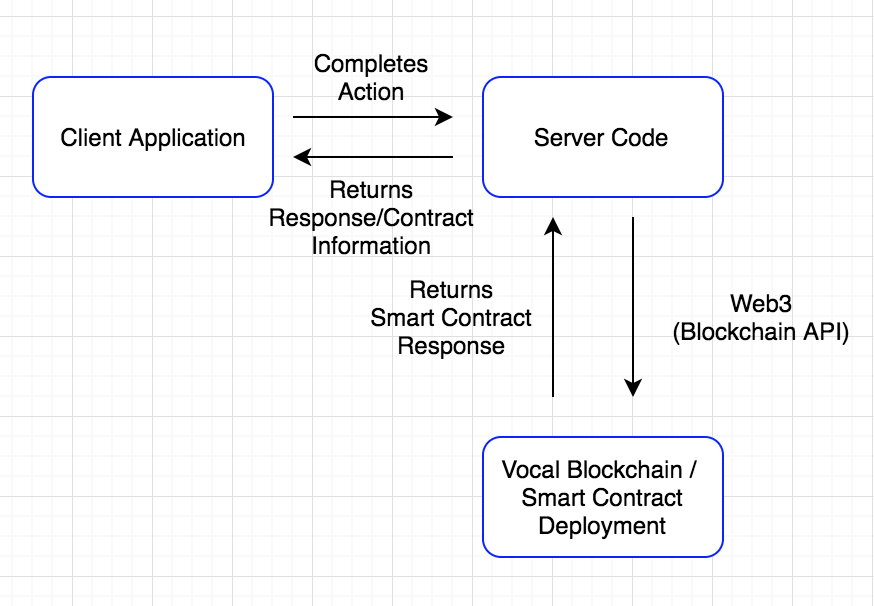
\includegraphics[width=8cm]{assets/architecture.png}
      \caption{Basic Vocal Client/Server Architecture}
      \centering
    \end{figure}

    % Vocal is deployed as a smart contract on the Ethereum.

    % \subsection{Limitations}
    % TODO:{discuss limitations of transactions per second on Ethereum}
    % TODO:{Address these counter arguments and others for the coin.}
    
    \section{Coin Supply}

   Vocal coin follows a fixed coin distribution model as to be described in this section.

    \subsection{Total Cap}
   Vocal will be capped at a total circulating supply of $100,000,000$ coins. Coins will be earned by engaging with advertisements (either by watching, viewing, or opening advertisements).
     The coin quantity earned for each action will vary according to the total number of supply still remaining. In this sense, viewing ads has become the notion of mining - rewarding users for participation on the network.

     As more coins are mined and held - the coin quantity reward granted will diminish; however, the corresponding market or redeemable value of the coin may correspondingly increase in value. This model lends itself similarly to Bitcoin. In that users
     will still be given roughly equivalent reward for the amount of work and early holders/participants will potentially be rewarded for their early entry point and involvement.

    \section{Distribution}

    The distribution of the coin will proceed as follows.

    \begin{enumerate}
    \item Vocal Launch (50\%)
   Vocal is inherently a publicly traded and earned coin that plays a critical role in the expansion of this new ad engagement platform. We are fully committed to creating a sound governance structure and we plan to dedicate significant resources to the continued Research and Development of the platform.
    \item Retained by Vocal Coin (15\%)
    The Vocal coin core development team will be able to sustain itself using funds raised through the coin launch. If the Vocal platform proves itself to be a fundamental technology as we believe it to be, the retained Vocal coins will allow the Vocal development team to sustain operations for many years.
    \item Developer Fund (15\%)
    The Developer Fund will be used to make targeted capital injections into high potential projects and teams that are attempting to grow the Vocal Coin ecosystem, strategic partnerships, hackathon prizes and community development activities.
    \item Founding Team (10\%)
    The founding team’s allocation of Vocal will vest over a traditional 4 year vesting schedule with a one year cliff. This is standard practice for equity vesting and we believe the same standards should be applied to the coin offering. 
    \item Early Backers and Advisors (10\%)
    Our backer and advisors are valuable resources to the expansion and growth of the Vocal platform. This remaining 10\% will be reserved for them, as a continued incentive to offer guidance and sustain a coin that holds genuine utility.
    \end{enumerate}
    
    % \subsection{Subsection Heading Here}
    % Subsection text here.
    % \subsubsection{Subsubsection Heading Here}
    % Subsubsection text here.


    \subsection{Challenges and Limitations}

    Creating an advertising-based currency poses several challenges. We highlight a few of them here; for example,

    \begin{enumerate}
      \item In order for advertisers to participate, the opportunity for them should be equal to or greater than current other opportunities and channels. 
      \item Is that true for participation in Vocal? For their participation, they would be both paying for Vocal and be willing to provide a good or service to a consumer in exchange for coins. How is this better than distributing coupon’s from a advertiser’s point of view?
      \item Why would an advertiser want coins? What do they do with them thereafter?
      \item The quality of the advertisement view is important to its value. For instance, if a user is watching ads continuously, the value of a single ad may not be necessarily very high. How does Vocal mitigate this? And how does this affect the go to market strategies for advertisers who wish to become involved with Vocal Coin?
    \end{enumerate}

    These are fundamental questions to be solved by our Roadmap below.
    
    \section{Development Roadmap}

    % https://tex.stackexchange.com/questions/196794/how-can-you-create-a-vertical-timeline

    \newcommand\ytl[2]{
    \parbox[b]{8em}{\hfill{\color{cyan}\bfseries\sffamily #1}~$\cdots\cdots$~}\makebox[0pt][c]{$\bullet$}\vrule\quad \parbox[c]{3cm}{\vspace{7pt}\color{red!40!black!80}\raggedright\sffamily #2.\\[7pt]}\\[-3pt]}
    \begin{table}
    \caption{Vocal Coin Timeline}
    \centering
    \begin{minipage}[t]{\linewidth}
    \color{gray}
    \rule{\linewidth}{1pt}
    \ytl{Nov 2017}{Finish coin proposal and development}
    \ytl{Dec 2017}{Finish Client facing coin application}
    \ytl{Jan 2018}{Vocal Coin Presale}
    \ytl{Apr 2018}{Mobile application released for Android}
    \ytl{Jul 2018}{Coins redeemable for goods and services}
    \ytl{Dec 2018}{Obtain retail partnerships for addition offers}
    \ytl{2019}{TBD: Ongoing security and product development}
    \bigskip
    \rule{\linewidth}{1pt}%
    \end{minipage}%
    \end{table}

    % \scalebox{1}{
    %   \begin{tabular}{r |@{\foo} l}
      
    %   2017 & \\
    %   September & Finish Development \\
    %   November & Coin Presale \\ 
    %   December & Public Coin Launch \\
    %   2018 & \\
    %   January & Accounting and Web Platform\\
    %   April & Android Mobile App released\\
    %   July & Coins redeemable for goods and services
    %   December & Obtain retail partnerships for additional offers \\
    %   2019 & \\
    %   January -> & TBD \\
      
    %   \end{tabular}
    % }
    % TODO:{Discussion of road map features and potential extensions of the protocol}
    
    \section{Conclusion}
   Vocal is a coin that has potential both as a store of advertising value and as an accounting system for advertisement engagement. Taking inspiration from both the Bitcoin and Ethereum mining models, one of Vocal's main goals is to create a coin ecosystem whose rewards stay consistent over time (but with greater potential for individual growth with a more early the entry point). The coin is designed to be easily accountable by transactions discoverable on the public ethereum (ERC20) blockchain.

   Vocal coin's initial offering will be done in early January 2018.

    % TODO:{Summarize Vocal objectives} 
    
    % conference papers do not normally have an appendix
    % use section* for acknowledgment
    \section*{Appendix}

    \subsection{Founding Team}
   Vocal was founded by Eric Asquith and Chris Buonocore. Eric is a Boston-area natives and bring a complimentary blend of professional experience to Vocal. He is also an attorney and real estate broker, with a clear vision for how technology can fix relationships between customers and advertisers. Chris is a former consultant and now developer from silicon valley with over 8 years of development experience. He brings wealth of relevant experience to take Vocal to consumers - holding expertise in creating and scaling mobile-based software platforms.  

    \subsection{Acknowledgements}

    We would like to express our gratitude to our mentors, advisors and to the many people in the Ethereum community that have been so welcoming and generous with their knowledge. 
    In particular, we would like to thank the folks in the Boston Cryptocurrency and Ethereum developers meetup groups for their support and advice.

    \subsection{ERC20 Vocal Protocol}
   Vocal follows the ERC20 (ethereum-blockchain) protocol for recording transactions.
    ERC20 establishes a standard contract ABI for coins on the Ethereum blockchain and has become the de facto representation for all types of digital assets. ERC20 coins share the same contract interface, simplifying integration with external contracts.
    Core ERC20 functions include:

    \begin{enumerate}
    \item transfer(to, value)
    \item balanceOf(owner)
    \item approve(spender, value)
    \item allowance(owner, spender)
    \item transferFrom(from, to, value)
    \end{enumerate}

    EIP101 includes a proposal to change ether to follow the ERC20 coin standard. For now, a “wrapper” smart contract may be used as a proxy for ERC20 ether. For reference, see the Maker implementation or the Gnosis implementation.
    \subsubsection{Contract ABI}
    EIP50 proposes an extension to the contract ABI to support structs. This would allow the community to establish standard Order and Signature data structures, simplifying our contract interface and integrations with external contracts.
    \subsubsection{Ethereum Name Service}
    EIP137 or Ethereum Name Service (ENS) will be used to resolve human-readable names, such as “myname.eth,” into machine-readable identifiers that may represent Ethereum addresses, Swarm and/or IPFS content hashes or other identifiers. It can also be used to associate metadata with names, such as contract ABIs or whois information. ENS will be used by 0x protocol to create more intuitive message formats that optionally reference Makers, Takers and Relayers by name.
    % \cite{Voit2012b}
 
    
    % trigger a \newpage just before the given reference
    % number - used to balance the columns on the last page
    % adjust value as needed - may need to be readjusted if
    % the document is modified later
    %\IEEEtriggeratref{8}
    % The "triggered" command can be changed if desired:
    %\IEEEtriggercmd{\enlargethispage{-5in}}
    
    % references section
    
    % can use a bibliography generated by BibTeX as a .bbl file
    % BibTeX documentation can be easily obtained at:
    % http://mirror.ctan.org/biblio/bibtex/contrib/doc/
    % The IEEEtran BibTeX style support page is at:
    % http://www.michaelshell.org/tex/ieeetran/bibtex/
    %\bibliographystyle{IEEEtran}
    % argument is your BibTeX string definitions and bibliography database(s)
    %\bibliography{IEEEabrv,../bib/paper}
    %
    % <OR> manually copy in the resultant .bbl file
    % set second argument of \begin to the number of references
    % (used to reserve space for the reference number labels box)
    % \begin{thebibliography}{1}
    
    % \bibitem{IEEEhowto:kopka}
    % H.~Kopka and P.~W. Daly, \emph{A Guide to \LaTeX}, 3rd~ed.\hskip 1em plus
    %   0.5em minus 0.4em\relax Harlow, England: Addison-Wesley, 1999.
    
    % \end{thebibliography}

    \printbibliography
    % \bibliography{mybib}{}
    % \bibliographystyle{plain}
   
    \end{document}
    
    
    